\subsection{About ktlint}
\par Ktlint is a popular an anti-bikeshedding Kotlin linter with built-in formatter created by pinterest. It tries to capture (reflect) official code style from kotlinlang.org and Android Kotlin Style Guide and then automatically apply these rules to your codebase. Ktlint checks and can automatically fix code and it claims to be simple and easy to use. Ktlint has been developing since 2016 and from then on it has 3.8k stars, 299 forks and 390 closed PRs (at least on the moment of writing this whitepaper). There have been written over 15k lines of code. Ktlint has it's own ruleset, which divides on standard and experimental rules. Ktlint can be used as a plugin via Maven or Gradle. To configure rules in Ktlint you should modify .editorconfig file. But you can't configure specific rules, instead you can provide some common settings. In other words, ktlint has a "fixed hardcoded" codestyle that is not very configurable. Properties should be specified under \textbf{[*.{kt,kts}]}. If you want to implement your own rules you need to create a ruleset. Ktlint is using java's ServiceLoader to discover all available "RuleSets". ServiceLoader is used to inject your own implementation of rules for the static analysis. In this case ktlint becomes a third-party dependency and a framework. Basically you should provide implementation of "RuleSetProvider" interface. Ktlint refers to article on \textbf{medium} \footnote{\url{https://medium.com/@vanniktech/writing-your-first-ktlint-rule-5a1707f4ca5b}}on how to create a ruleset and a rule.
\par A lot of projects uses ktlint as their code formatting tool. For example, OmiseGo \footnote{\url{https://github.com/omgnetwork/android-sdk}} (currently rebranding to OMG Network) - a quite popular cryptocurrency.

\subsection{About detekt}
\par Detekt is a static code analysis tool. It operates on an abstract syntax tree provided by Kotlin compiler and, on top of that, they do complex analysis of code. However, this project is more focused on checking rather than fixing. Similarly to ktlint, it has it's own rules. Detekt uses wrapped ktlint to redefine rules as it's formatting rules. Detekt supports such features as code smell analysis, highly configurable rule sets, IntelliJ integration, third-party integrations for Maven, Bazel and Github actions, mechanism for suppression of their warnings with @Suppress annotation and many more. It is being developed since 2016 and today it has 3.2k stars, 411 forks and 1850 closed PRs. It has circa 45k lines of code.
\par Detekt is used in such projects as fountain or Kaspresso. "Fountain is an Android Kotlin library conceived to make your life easier when dealing with paged endpoint services" \footnote{\url{https://github.com/xmartlabs/fountain}} and Kaspresso is a framework for UI testing on Android made by KasperskyLab \footnote{\url{https://github.com/KasperskyLab/Kaspresso}}.

\subsection{About ktfmt}
\par Ktfmt is a program that formats Kotlin code, based on google-java-format. It's development has started in Facebook in the end of 2019. It can be added to your project through a Maven dependency, Gradle dependency, IntelliJ plugin or you can run it through a command line. Ktfmt is not a configurable application, so to change any rule logic you need to download the project and redefine some constants. Ktfmt has 214 stars, 16 forks, 20 closed PRs and around 7500 lines of code. 

\subsection{About diKTat}
\par Diktat as well as ktlint and detekt is a static code analysis tool. But diktat is not only a tool, but also coding convention (link) that in details describes all the rules that you should follow when writing a code on Kotlin. It's development has started in 2020 and at the time of writing this whitepaper diKTat has 130 stars and 12 forks. DiKTat operates on AST provided by kotlin compiler. 
\par So why is diKTat better? First of all, we support much more rules than ktlint. Our ruleset includes more than 100 rules, that can both check and fix your code. Second, diKTat is configurable. A lot of rules have their own settings, and all of them can be easily understood. For example, you can choose whether you need a copyright, choose a length of line or you can configure your indentations. A little more about indentations, in this rule you can specify indentation size, whether you need a new line at the end or specify if you need aligned parameters. Third, diKTat is very easy to configure. You don't need to spend hours only to understand what each rule is doing. Our ruleset is a yml file, where each rule is commented out with the description. Last but not the least, diKTat can be used as a CI/CD tool in order to avoid merging errors in the code.
\par Overall it can find code smells and code style issues. Also it can find pretty unobvious bugs by complex AST analysis.

\subsection{A few words about Jetbrains}
\par Jetbrains created one of the best IDEs for Java and Kotlin called IntelliJ. This IDE supports a built-in linter. However it is not a well-configurable tool, you are not able to specify your own coding convention and it is not useful for CI/CD as it is highly coupled with UI. Unfortunately such static analysis is not so effective as it cannot prevent merging of the code with bugs into the repository. As experience shows - many developers simply ignore those static analysis errors until they are blocked from merging their pull requests.

\subsection{Graphics}
\subsubsection{Detekt Code Frequency}
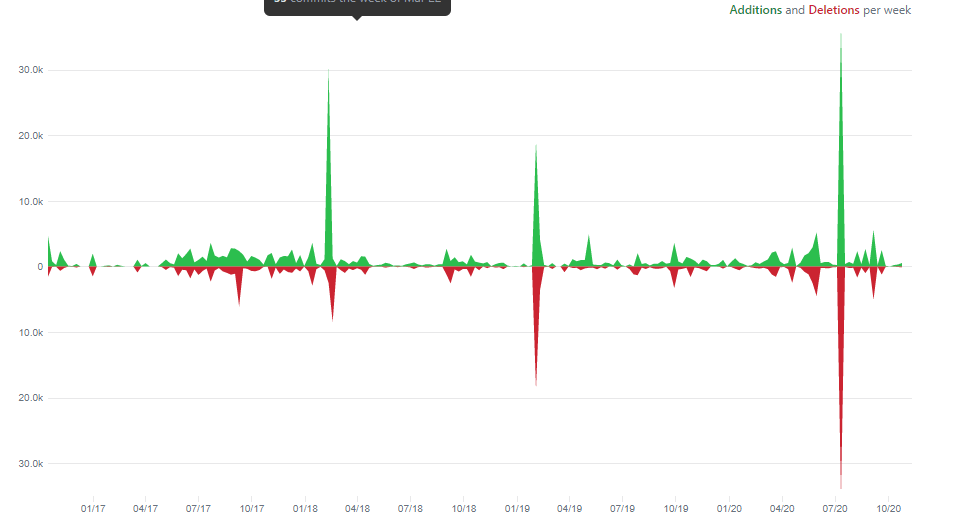
\includegraphics[scale=0.6]{pictures/detekt.png}
\subsubsection{Ktlint Code Frequency}
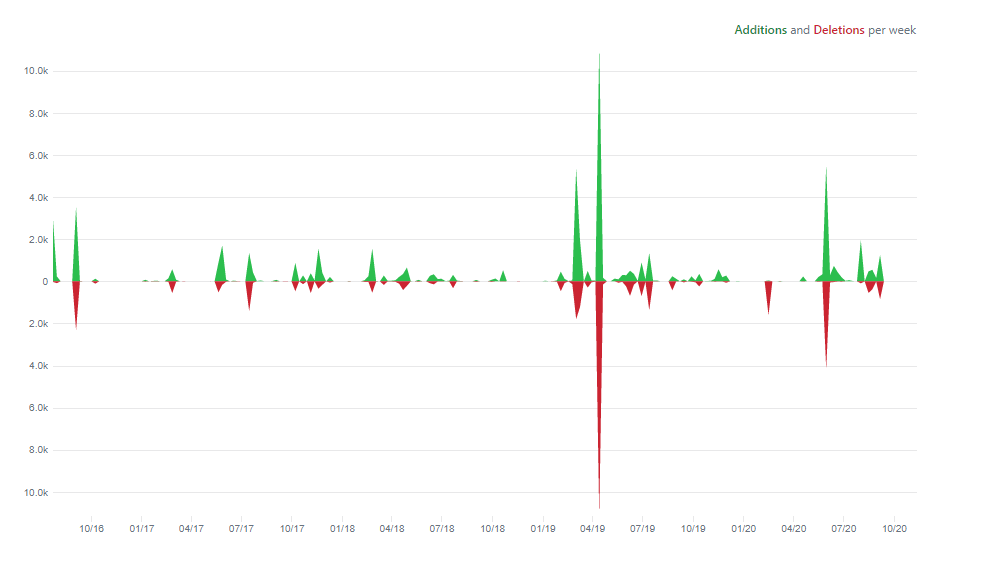
\includegraphics[scale=0.6]{pictures/ktlint.png}
\subsection{Ktfmt Code Frequency}
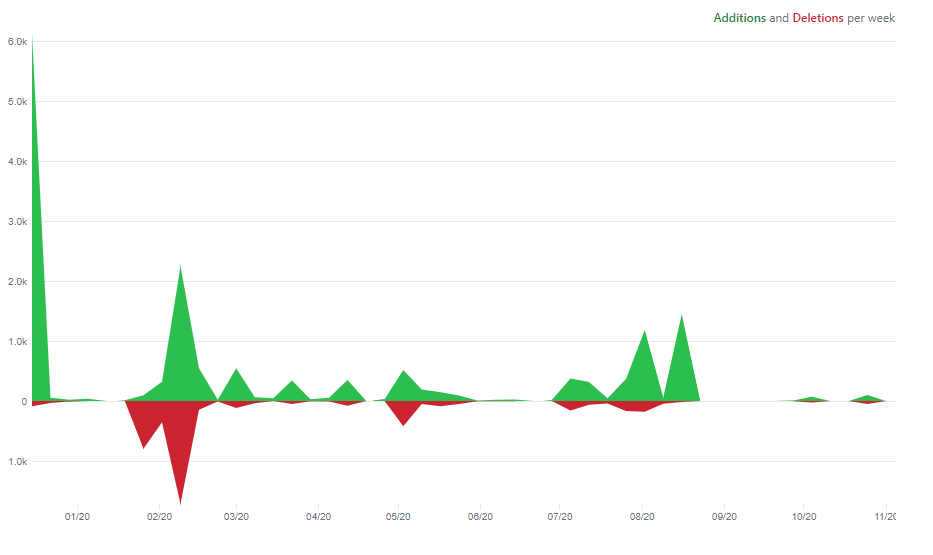
\includegraphics[scale=0.6]{pictures/ktfmt.png}
\subsubsection{DiKTat Code Frequency}
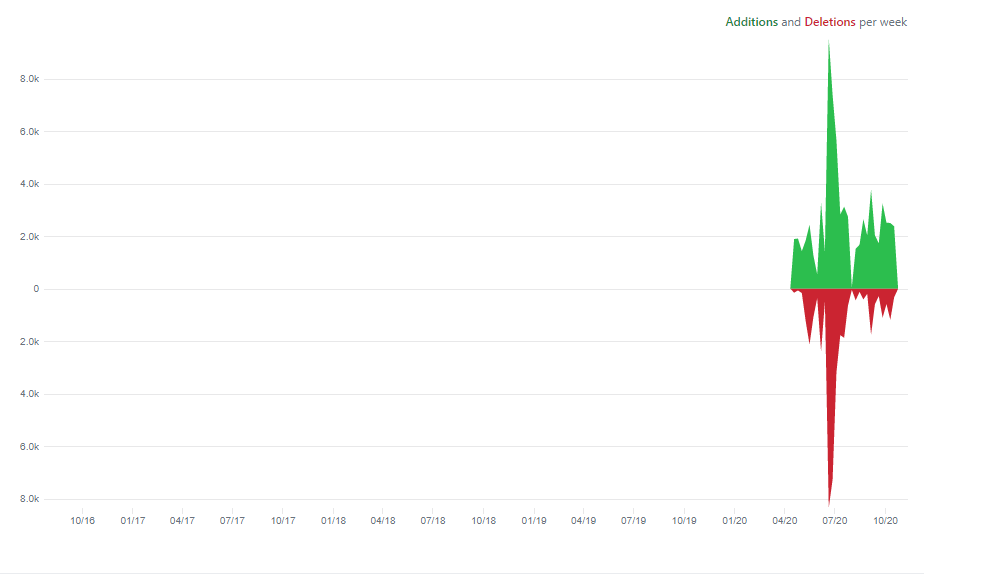
\includegraphics[scale=0.6]{pictures/diktat.png}
\subsection{Summary}

\begin{center}
\begin{tabular}{ |p{3cm}|p{3cm}|p{3cm}|p{3cm}|p{3cm}|  }
\hline
\multicolumn{5}{|c|}{\textbf{Comparing table}} \\
\hline
& diKTat& ktlint &detekt & ktfmt \\
\hline
starting year & 2020 & 2016 & 2016 & 2019 \\
stars & 130 & 3.2k & 3.8k & 214\\ 
forks & 12 & 299 & 411 & 16\\
closed PRs & 226 & 390 & 1850 & 20 \\
lines of code & 22k & 15k & 45k & 7,5k\\
number of rules & $>$100 & $\approx$ 20 & $>$100 & $\approx$ 10 \\
\hline

\hline
\end{tabular}
\end{center}